\chapter{Метод обучения стратегии для управления движением
шагающего робота с заданной линейной и угловой скоростью}\label{ch:ch3}

\section{Постановка задачи управления шагающим роботом}

%\begin{figure}[ht]
%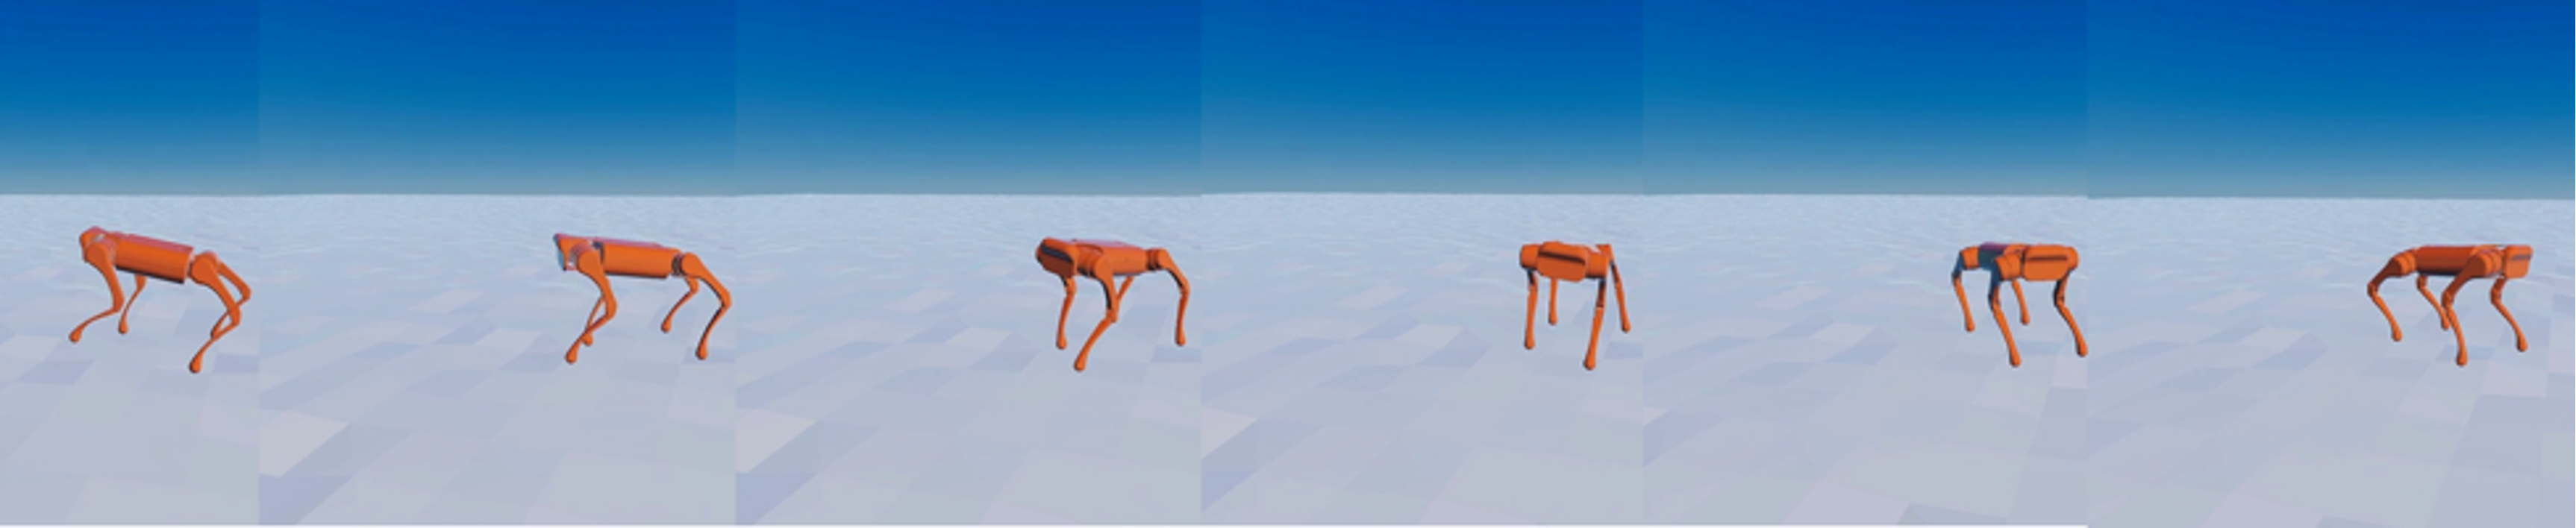
\includegraphics[width=1\textwidth]{images/turn.png%}
%\caption{Unitree A1 robot, “turn counterclockwise” %task.}
%\label{fig:turn}
%\end{figure}

\begin{figure}[ht]
    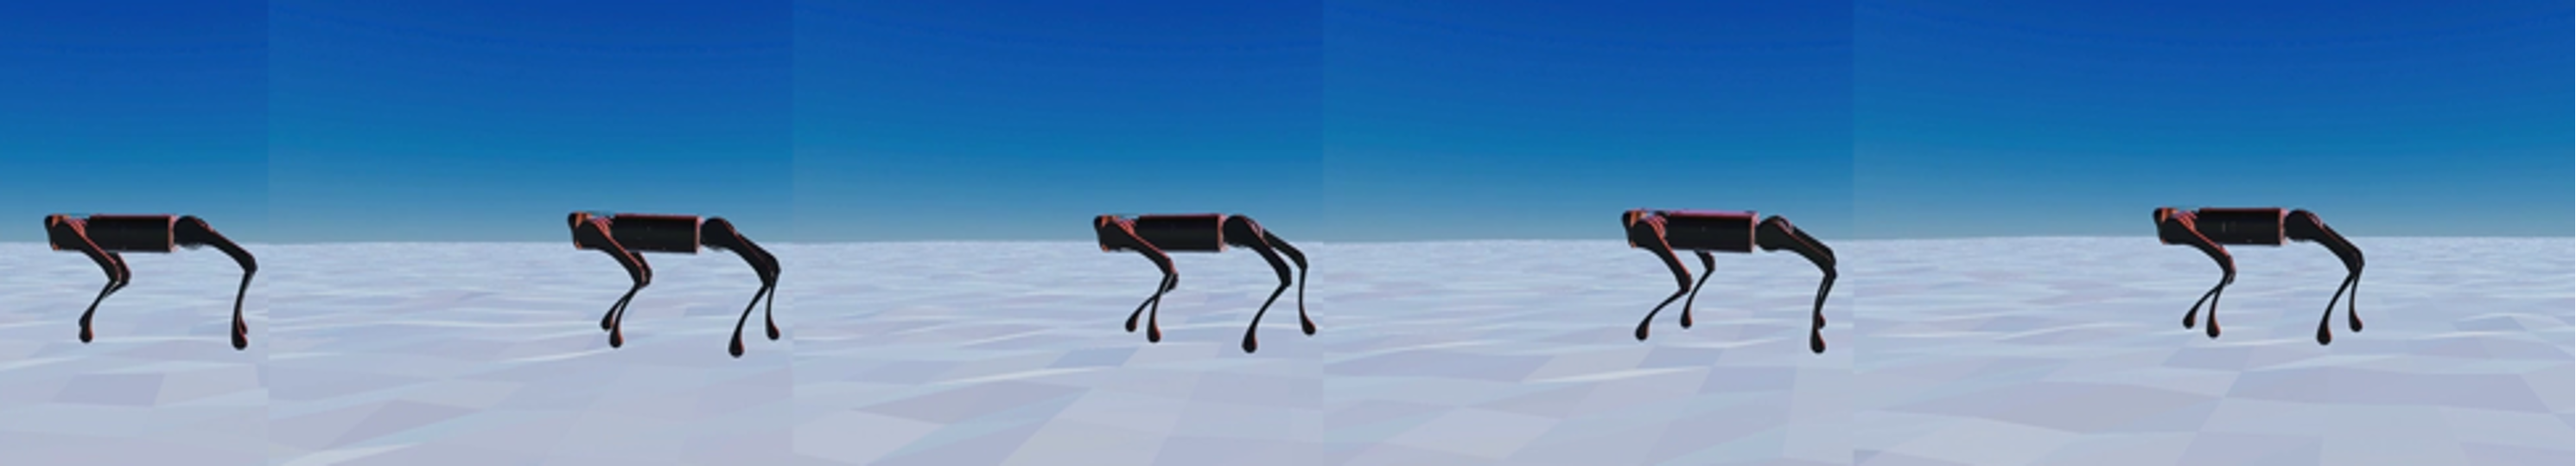
\includegraphics[width=1\textwidth]{images/move_forward.png}
    \caption{Unitree A1 робот, задача ``Движение вперед''}
    \label{fig:mv_forward}
\end{figure}

%\begin{figure}[ht]
%\includegraphics[width=1\textwidth]{images/move_bac%kward.png}
%\caption{Unitree A1 robot, “move backward” task.}
%\label{fig:mv_backward}
%\end{figure}

Робототехника является одним из наиболее важных применений обучения с подкреплением. Роботы, способные адаптироваться к изменяющимся условиям окружающей среды, будут иметь множество применений в коллаборативной робототехнике \cite{levine2016end} и автономном вождении \cite{kiran2021deep}. В обучении с подкреплением робот взаимодействует со средой и выучивает стратегию, которая максимизирует суммарную дисконтированную награду, получаемую в течении эпизода.  Этот подход имеет существенные преимущества перед классическими методами управления, так как агент может самостоятельно выучить оптимальную последовательность действий опираясь только на скалярную функцию награды. Функцию награды в большинстве задач задать сильно проще, чем определить оптимальную последовательность действий агента. Однако из-за того, что робот взаимодействует со средой методом проб и ошибок, метод обучения с подкреплением имеет ряд сложностей. Во-первых, процесс обучения требует большого количества данных для того, чтобы выучить оптимальную стратегию. Во-вторых, не аккуратно заданная функция награды может привести к тому, что агент выучит не безопасные действия, которые могут повредить робота или будет действовать не оптимально. В-третьих, при переносе стратегии, обученной в симуляции на физического робота, стратегия может работать не оптимально из-за разницы в наблюдениях. 

Задача управления движением шагающего робота с большим количеством степеней свободы достаточно сложна. Оптимальная стратегия должна хорошо фильтровать шумы в наблюдениях, не требовать чрезмерно большого количества данных для обучения и 
не совершать действий, которые могли бы повредить роботу. Так как не все желаемые характеристики стратегии могут быть достигнуты одновременно, в различных работах делается упор на разные свойства. В работе \cite{yang2020data} авторы представили подход, основанный на модели среды, который позволяет обучить стратегию с использованием только 4.5 минут дынных, собранных на шагающем роботе, что соответствует 45000 шагов агента. В работе \cite{Hwangbo2019} авторы обучили шагающего робота ANYmal \cite{anymal}, используя алгоритм обучения с подкреплением PPO \cite{Schulman2017ProximalPO} с обучением по расписанию и добавлением шумов в наблюдения, благодаря чему обученная стратегия смогла успешно управлять физическим роботом. В  \cite{chalter} авторы для обучения стратегии использовали двух агентов: учителя и ученика. Стратегия учителя имела доступ к привилегированной информации такой, как коэффициент трения, сила реакции опоры.  Стратегия ученика не имела доступа к этой информации и обучалась повторять стратегию учителя. В работе \cite{rapid} авторы обучили стратегию для управления движением робота MIT Mini Cheetah с высокой скоростью, используя обучение по расписанию.

В рамках данной работы был разработан подход для управления движением робота Unitree A1 \cite{unitree}, основанный на обучении с подкреплением. Обучение стратегии для управления роботом производится в симуляции. При обучении стратегии используется расписание, постоянно увеличивающее сложность текущей задачи. Для обучения стратегии была разработана функция награды, которая побуждает агента выучивать безопасное и плавное движение с заданной скоростью. Также, для того, чтобы выучить устойчивую стратегию, во время обучения в наблюдения добавлялись шумы. 

\section{Метод управления линейной и угловой скоростью шагающего робота основанный на обучении с подкреплением}

В работе использовалась модель робота Unitree A1, показанная на рис.~\ref{fig:mv_forward}. Робот имеет четыре конечности и обладает 12 степенями свободы ---  по три сустава на каждую из четырех конечностей. Для симуляции динамики робота использовался симулятор Raisim~\cite{raisim}. Для обучения и тестирования агента был выбран следующий набор задач: 

\begin{itemize}
    \item ``Движение вперед''.
	\item ``Движение вперед с заданной скоростью''.
    \item ``Движение назад''.
    \item ``Поворот по часовой стрелке''.
    \item ``Поворот против часовой стрелки''.
\end{itemize}

\paragraph{Пространство состояний.} Пространство состояний имеет размерность 49 и включает в себя текущую высоту туловища робота (1), ориентацию робота в пространстве --- углы крена и тангажа (2), положения суставов робота (12), скорости суставов робота (12), предыдущие положения суставов (12), линейные (3) и угловые (3) скорости робота, индикаторы контакта конечностей с поверхностью (4). Для задачи ``Движение вперед с заданной скоростью'' наблюдение также включает в себя 50 измерение ---  целевую скорость. Наблюдение нормализуется с использованием константного значения среднего и дисперсии.

\paragraph{Пространство действий.} Пространство действий является непрерывным и имеет размерность 12. Действиями агента являются следующие положения суставов робота. Действия также нормализованы на постоянное среднее значение и дисперсию.  

\paragraph{функция награды.} Была разработана функция награды, состоящая из 9 слагаемых, с коэффициентами, приведенными в таблице \ref{tab:rcoeff}:

\begin{multline}
    r = k_{torso\ height} \cdot r_{torso\ height} +
    k_{torque} \cdot r_{torque} +\\
    k_{joint\ speed} \cdot r_{joint\ speed} +
    k_{slip} \cdot r_{slip} +\\
    k_{work} \cdot r_{work} + 
    k_{ground\ impact} \cdot r_{ground\ impact} +\\
    k_{z\ acceleration} \cdot r_{z\ acceleration} +  k_{velocity} \cdot r_{velocity} +\\
    k_{transverse\ and\ rotation} \cdot r_{transverse\ and\ rotation}
\label{eq:unitree_reward}
\end{multline}


Для определения слагаемых, использовавшихся в функции награды, воспользуемся следующими определениями: 
 $k_c$ - коэффициент, определяющий сложность задачи в обучении по расписанию, $h_0$ – высота туловища робота в начале эпизода, $h$ – текущая высота туловища робота, $\tau$ - крутящий момент в суставе, $\tau_p$ – предыдущее значение крутящего момента в суставе, $\lVert \rVert$ - L2 норма, $V_t$ - линейная скорость туловища робота, $W$ - угловая скорость, $\hat{\cdot}$ - целевое значение переменной, $V_j$ - линейная скорость суставов робота, $V_{ft}$ - тангенциальная скорость стопы робота (x, y компоненты), $x_j$ линейное положение суставов, $x_{pj}$ предыдущее положение суставов, $F_f$ – сила реакции опоры между поверхностью и стопой, $F_{pf}$ – сила реакции опоры на предыдущем шаге, $D$ – направление равное 1 или -1, нижний индекс x,y,z соответствует одной из компонент вектора. 

Первые семь компонент в уравнении \ref{eq:unitree_reward} не зависят от задачи и используются для задания гладкой и безопасной стратегии. Они определяются следующим образом:

$$
r_{torso\ height}= k_c \cdot (h-h_0)^2
$$
$$
r_{torque} = k_c \cdot \lVert \tau \rVert ^2
$$
$$
r_{joint\ speed}= k_c \cdot \lVert V_j \rVert ^2
$$
$$
r_{slip} = k_c \cdot(\lVert V_{ft} \rVert ^2+ W_z^2)
$$
$$
r_{work}= k_c \cdot |\tau^T \cdot (x_j-x_{pj})|
$$
$$
r_{ground\ impact} = k_c \cdot \lVert F_f-F_{pf} \rVert ^2
$$
$$
r_{z\ acceleration}= k_c \cdot V_z^2
$$

В задачах ``Движение вперед'' и ``Движение назад'' $r_{velocity}$ и $r_{transverse\ and\ rotation}$ определены следующим образом: 

$$
r_{velocity} = \mathrm{clip}(V_x \cdot D / \hat{V_x}, 0, 1)
$$
$$
r_{transverse\ and\ rotation}= k_c \cdot (V_y^2+W_z^2)
$$

В задаче ``Движение вперед с заданной скоростью'' $r_{velocity}$ и $r_{transverse\ and\ rotation}$: 

$$
r_{velocity} = \max(1 - |V_x / \hat{V_x} - 1|, 0)
$$
$$
r_{transverse\ and\ rotation}= k_c \cdot (V_y^2+W_z^2)
$$

В задачах ``Поворот по часовой стрелке'' и ``Поворот против часовой стрелки'' $r_{velocity}$ и $R_{transverse\ and\ rotation}$: 

$$
r_{velocity} = \mathrm{clip}(W_z \cdot D / \hat{W_z}, 0, 1)
$$
$$
r_{transverse\ and\ rotation}= k_c \cdot (V_x^2+V_y^2)
$$

\paragraph{Шумы}. Для того чтобы полученная стратегия была устойчива к шумам, мы добавляем следующие шумы в процессе обучения: центр масс робота выбирается из распределения $COM \sim k_c \cdot U(-0.0015, 0.0015)$, где $U(A,B)$ равномерное распределение от $A$ до $B$, коэффициент трения $k_f \sim 0.875 + k_c \cdot U(0.5, 1.25)$, крутящий момент $k_m \sim 1 + k_c \cdot U(0.9, 1.1)$, применяем силу в $1000\ N$ (что эквивалентно  ускорению 8.2g для робота весом 12.5kg) в случайном направлении к туловищу робота с вероятностью 0.5 на каждом шаге и также применяем случайный момент сил  в 100 $N \cdot m$ с вероятностью 0.05. 

\paragraph{Расписание}. Для обучения стратегии используется расписание с коэффициентом  $k_c$, монотонно растущим от $0$ до $1$ в течение процесса обучения. Благодаря этому агент вначале обучения учится решать простые задачи и затем постепенно адаптируется к задачам большей сложности.

\begin{table} [htbp]
    \centering
    \begin{threeparttable}
        \caption{Коэффициенты функции награды.}\label{tab:rcoeff}
        \begin{tabular}{| p{8cm} || p{8cm} |}
            \hline
            \hline
            коэффициент & значение \\
            \hline
            $k_{velocity}$ &	1.25 \\
            $k_{lateral\ and\ rotation}$ &	-0.9 \\
            $k_{height}$	& -1.0 \\
            $k_{torque}$	& -0.0005 \\ 
            $k_{joint\ speed}$ &	-0.0015 \\
            $k_{slip}$ &	-0.1 \\
            $k_{work}$ &	-0.125 \\
            $k_{ground\ impact}$ &	-0.000015 \\
            $k_{z\ acceleration}$ &	-2.0 \\
            \hline
            \hline
        \end{tabular}
    \end{threeparttable}
\end{table}


В качестве основной части в алгоритме обучения стратегии выступает алгоритм PPO~\cite{Schulman2017ProximalPO}. Для стабилизации процесса обучения скорость обучения (learning rate) на каждом шаге обучения стратегии регулируется с использованием kl-дивергенции между распределениями действий на текущем и предыдущем шагах:

\begin{equation}
  lr_{t+1} =
    \begin{cases}
      lr_t / 2 & \text{если $kl(\pi_{\theta^{\prime}}, \pi_{\theta}) > 2 \cdot kl_{target}$ }\\
      lr_t \cdot 2 & \text{если $kl(\pi_{\theta^{\prime}}, \pi_{\theta}) < kl_{target} / 2$ }\\
      lr_t & \text{иначе}
    \end{cases}     
\end{equation}
$kl_{target}$ --- целевое значение kl-дивергенции. Максимальная длинна эпизода равна \textbf{3500 шагов}. Такой длинны эпизода достаточно для того, чтобы агент достиг границы симуляционной среды к концу эпизода. Параметры алгоритма PPO, использованные в работе, приведены в таблице~\ref{tab:ppoparams}.

\begin{table} [htbp]
    \centering
    \begin{threeparttable}
        \caption{Параметры алгоритма PPO.}\label{tab:ppoparams}
        \begin{tabular}{| p{8cm} || p{8cm} |}
            \hline
            \hline
            параметр & значение \\
            \hline
            clipping parameter &	0.2 \\
            gamma &	0.998 \\
            lambda &	0.95 \\
            value loss coefficient &	0.5 \\
            entropy coefficient &	0.0 \\
            learning rate &	0.0005 \\
            maximum gradient norm &	0.5 \\
            desired kl divergence &	0.01 \\
            \hline
            \hline
        \end{tabular}
    \end{threeparttable}
\end{table}

При реализации нейронных сетей актора и критика использовались полносвязные нейронные сети с двумя скрытыми слоями по $512$ нейронов в каждом. 

\section{Оценка результатов работы в симуляции}

При обучении агента в симуляции использовалось $100$ копий среды, запущенных параллельно. Обновление параметров нейронных сетей производилось каждые 128 шагов среды с помощью алгоритма обратного распространения ошибки и оптимизатора Adam~\cite{kingma2014adam}. Полное число обновлений равно $5000$. Тестирование обученного агента производилось в симуляции на $100$ эпизодах. Результаты тестирования приведены в таб.~\ref{tab:unitree_eval} и на рис.~ \ref{fig:unitree_eval_forward}. В таблице \ref{tab:unitree_eval} приведены результаты тестирования обученного агента для задач ``Движение вперед'', ``Движение назад'', ``Поворот по часовой стрелке'' и ``Поворот против часовой стрелки''. Видно, что для задач ``Движение вперед'', ``Движение назад'' стратегия более стабильна и число шагов близко к максимальной длине эпизода. В задачах ``Поворот по часовой стрелке'' и ``Поворот против часовой стрелки'' выученная стратегия менее стабильна, что приводит к меньшей суммарной награде и меньшему среднему числу шагов. Причиной этому может служить то, что случайная сила дестабилизирует поворачивающегося агента больше, чем движущегося прямо.

\begin{figure}[ht]
\begin{subfigure}{.5\textwidth}
  \centering
  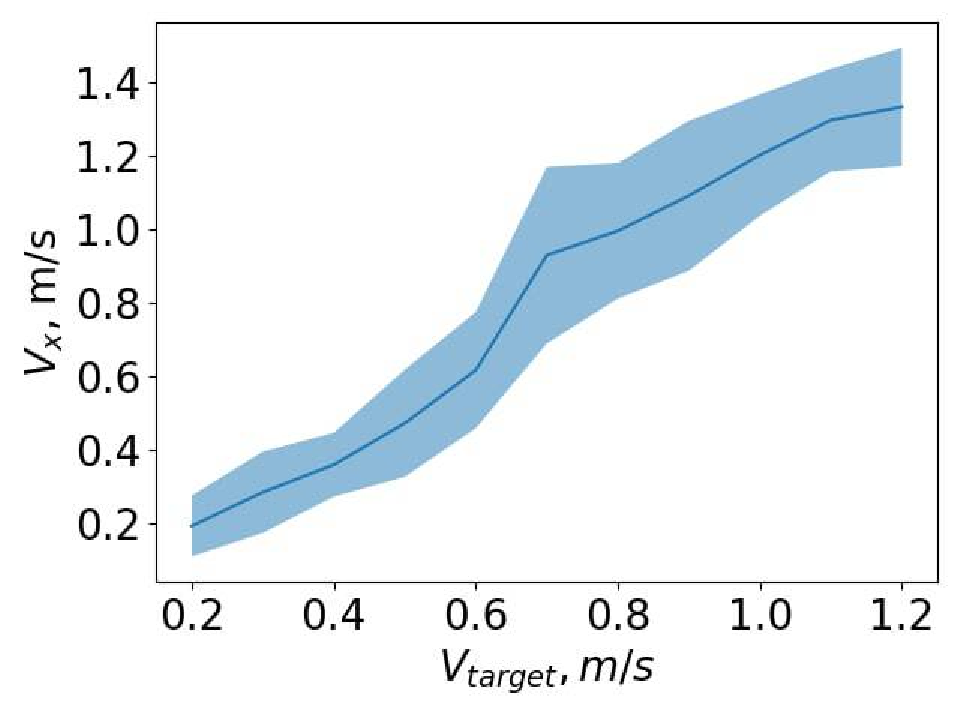
\includegraphics[width=1\textwidth]{images/vx}
\end{subfigure}%
\begin{subfigure}{.5\textwidth}
  \centering
  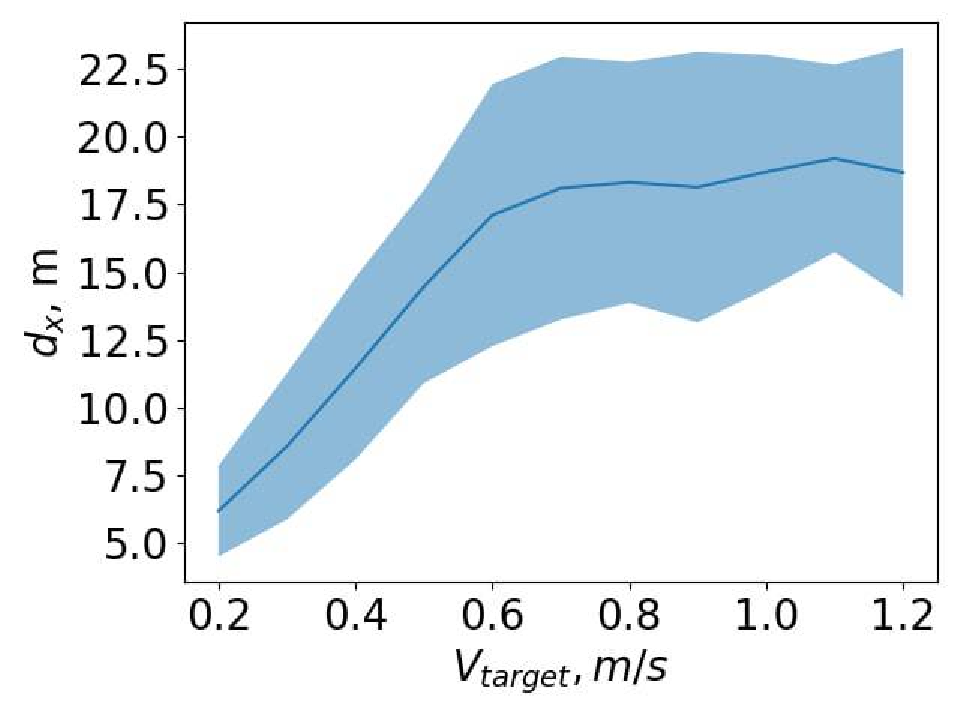
\includegraphics[width=1\textwidth]{images/dx}
\end{subfigure}%
\caption{Тестирование задачи ``Движение вперед с заданной скоростью''. (a) Скорость робота $V_x$ как функция целевой скорости $V_{target}$. (b) Расстояние пройденное роботом к концу эпизода $d_x$ как функция целевой скорости $V_{target}$.}
\label{fig:unitree_eval_forward}
\end{figure}

На рис.~\ref{fig:unitree_eval_forward} представлены результаты тестирования обученной стратегии в задаче ``Движение вперед с заданной скоростью''. Из рис.~\ref{fig:unitree_eval_forward}a видно, что обученный агент способен двигаться с различной скоростью и его скорость близка к целевой скорости. Расстояние, пройденное агентом вдоль оси $x$, показано на рис.~\ref{fig:unitree_eval_forward}b. При целевой скорости $V_{target} \in$ (0, 0.6) м/с расстояние, пройденное к концу эпизода, растет. При целевой скорости больше 0.6 м/с пройденное расстояние практически постоянно и равно расстоянию от агента до края среды.

\begin{table} [htbp]
    \centering
    \begin{threeparttable}
        \caption{Результаты тестирования обученного агента в симуляции.}\label{tab:unitree_eval}
        \begin{tabular}{| p{3cm} || p{3cm} | p{3cm} | p{3cm} |p{3cm} |}
            \hline
            \hline
            Задача & Движение вперед & Движение назад & Поворот по часовой стрелке & Поворот против часовой стрелки \\
            \hline
            Суммарная награда &	529 $\pm$ 124 &	508 $\pm$ 98 &	85 $\pm$ 219 &	165 $\pm$ 155 \\
            Число шагов & 3263 $\pm$ 633 &	3136 $\pm$ 545 &	2057 $\pm$ 1208 &	2095 $\pm$ 1325 \\
            \hline
            \hline
        \end{tabular}
    \end{threeparttable}
\end{table}

Полученные результаты показывают, что линейной и угловой скоростью робота Unitree A1 с хорошим качеством можно управлять с помощью обучения с подкреплением. 

\section{Выводы}

В рамках данной работы был предложен метод, позволивший обучить робота Unitree A1 решать различные задачи перемещения. Разработанная функция награды побуждает агента следовать плавной и безопасной стратегии. Результаты тестирования обученного агента показали, что он способен хорошо выполнять поставленные задачи в симуляции. В дальнейшем, стратегии, обученные для решения различных задач, могут быть объединены в одну стратегию, способную перемещаться с произвольной линейной и угловой скоростью. Затем данная стратегия может быть использована в качестве стратегии первого уровня в иерархическом методе обучения с подкреплением. Благодаря этому стратегия второго уровня сможет решать более сложные задачи, такие как перемещение грузов в заданную точку и обход препятствий. 



\clearpage
